%
% File acl2014.tex
%
% Contact: koller@ling.uni-potsdam.de, yusuke@nii.ac.jp
%%
%% Based on the style files for ACL-2013, which were, in turn,
%% Based on the style files for ACL-2012, which were, in turn,
\documentclass[10pt]{article}
\usepackage{report}
\usepackage{times}
\usepackage{url}
\usepackage{latexsym}
\usepackage{amsmath}
\usepackage{graphicx}
\usepackage{comment}
\usepackage{cite}

%\setlength\titlebox{5cm}

% You can expand the titlebox if you need extra space
% to show all the authors. Please do not make the titlebox
% smaller than 5cm (the original size); we will check this
% in the camera-ready version and ask you to change it back.


\title{Large-Scale Dataset Name Recognition by Semi-Supervised Learning}

\author{Jinfeng Rao\\
  Department of Computer Science \\
  University of Maryland \\
  {jinfeng@cs.umd.edu} \\\And
  Xing Niu \\
  Department of Computer Science \\
  University of Maryland \\
  {oxstar@cs.umd.edu} \\}

\date{}

\begin{document}
\maketitle
\begin{abstract}
%In some fields with no existing, widely-used benchmarks, finding appropriate datasets for experiments becomes a essential step in conducting research. Under these circumstances, a platform for storing dataset metadata, i.e, name, keyword, description, can be utilized for dataset inquiry and recommendation. 
In this paper, we leverage linguistic tools to solve the problem of dataset extraction from scientific literatures. We attempted three different approaches for extracting dataset from texts: classifier, dependency tree and conditional random fields(CRF). We evaluated these three approaches on a real world dataset, and got F1-Measure score higher as 70\%. Based on these work, we purposed a novel framework to extend conditional random fields in semi-supervised learning way by given a set of seeds(labeled datasets) as start point, and then iteratively find new datasets and patterns to bootstrap the learning process. The experiment results show the F1-Measure score continues increasing as the bootstrap process repeats.  
\end{abstract}
\section{Introduction}
Dataset selection is a fundamental problem when conducting research. Currently, most researchers tends to use some public benchmarks or datasets from related literatures to conduct experiments. However, in some fields with no existing benchmarks or publicly accessible datasets, researchers need to follow the dataset collection descriptions in related literatures to get the data, or sometimes difficult to obtain the exact datasets. These phenomena are rather common in realistic, leading to inconsistency of datasets in experiments and further resulting in performance incomparability of different work. Thus, a dataset platform, which permits researchers to search and download datasets, will simplify the problem of choosing and collecting appropriate datasets.    

Under such a situation, several dataset repositories have been developed and made public to researchers. For example, the KEEL\footnote{http://sci2s.ugr.es/keel/datasets.php} dataset repository and the UCI Machine Learning Repository\footnote{http://archive.ics.uci.edu/ml/} provide access to several hundred datasets in machine learning domain. The datasets in these repositories are most collected and maintained by manual work. However, collecting and integrating dataset sources mutually from the vast number of data sources, e.g, literatures, web, P2P sensor, is impractical. For constructing such platform automatically, \emph{dataset name recognition} is the first step to be solved. A more realistic scenario is to extract datasets from documents adaptively in a semi-supervised way by giving a set of labeled datasets as initial point. A standard way of semi-supervised learning is to start with a small set of seed items( in this case, labeled datasets) and iteratively grow it by finding contextual patterns that extracts the set of seeds from the texts, then identify a larger set of seeds through the contextual patterns, finally pick the best subset of candidate seeds and add to previous seeds. This iterative learning process is also called bootstrap learning. In this paper, we first attempted two different approaches for extracting dataset from texts: classifiers, conditional random fields (Lafferty et al. 2001). Both word-level features and contextual pattern features are employed. We used dependency tree to construct the contextual-level features for classifier methodologies. Then we purposed a novel bootstrapping framework for conditional random fields to guide the iterative learning process. This framework directs how to select a relatively better set of new seeds from all candidate seeds and how to adaptively train the CRF using intermediate statistics in the end of each iteration. \\

In conclusion, our contributions includes,
\begin{itemize}
\item Compared with the very limited work in dataset extraction, we tried three different linguistic approaches to solve this problem, and the efficiency is verified by experiments on real-world data.
\item We purposed an original bootstrapping framework for conditional random fields, which includes an evaluation metric called \emph{feature contribution score} for measuring the contribution of this feature to find new contextual patterns, and an incremental training algorithm to avoid retraining of CRF in the iteratively learning process. 
\end{itemize}

\section{Problem Definition and Workflow}
Given a corpus of research papers C, our objective is to find the dataset list $D = \{ d_1, d_2...d_n\}$ from the papers in the corpus. A paper usually contains multiply datasets, and we consider datasets with the same name in different papers as different instances. Consider a concrete example below: 
\begin{itemize}
\item The \textbf{DBLP} dataset contains 123k authors and 200k papers. 
\item Five of the sets in this subsection are from the UCI repository \#REF\# ( \textbf{iris} , \textbf{wine} , \textbf{pendigits} , \textbf{waveform} , \textbf{segmentation} ).
\end{itemize}
The dataset names are in bold form. In the first example, it is relatively simple to identify the dataset \textbf{DBLP} by employing some heuristic rules (i.e, like a candidate dataset is followed by keyword 'dataset'). For the second example, however, there are not much apparent heuristic rules to recognize 
the datasets. In these cases, an approach employing the contextual pattern information can be more efficient. In this section, we introduce our attempts of building classifier and structural prediction(CRF) to incorporate both word-level features and contextual pattern information. Before discussing the approaches, a brief introduction of preprocessing workflow is provided. 

\noindent \textbf{Workflow.} \\
The preprocessing workflow consists of following phases:
\begin{enumerate}
\item \textbf{Data Preparation.} Most research literatures are copyrighted, and we are not allowed to download too many articles from subscribed database (e.g. IEEE Xplore\footnote{http://ieeexplore.ieee.org/Xplore/home.jsp}, ACM Digital Library\footnote{http://dl.acm.org/}) in a short period of time via our university's library. We tried an alternative solution that used a Web crawler to dump articles from academic search engines such as Google Scholar\footnote{http://scholar.google.com/}.
\item \textbf{File Format Conversion.} Working with pdf file directly makes difficult to parse, extract and analysis of contents. We convert the research papers in \emph{pdf} format to raw texts. It's worth noting some format information will lost in this phase, like \emph{italic} form. 
\item \textbf{Content Positioning.} Dataset information are likely to appear in the experiment section. We reduce the contents to the paragraphs with occurrence of keywords 'dataset' or 'data set' in experiment section.
\item \textbf{Preprocessing.} The contents are tokenized before processing. Some frequent patterns are replaced by a uniform representation, e.g, all references are replaced by word '\#REF\#', all numeric words are replaced by '\#NUMBER\#'. 
\item \textbf{Candidate Generation.} We use some relaxed heuristic rules to generate candidate datasets in order not to miss any true datasets. A concrete example is to use following regular expression: \\
\textit{(The $|$ the $|$ a $|$ an) .\{3,30\} (dataset $|$ data)} \\
This regular expression extracts all words or phrases as candidates with length in [3,30], previous word is any keyword of \{\textit{The, the, a , an}\} and followed word is any keyword of \{\textit{dataset, data}\}. For each candidate, we extract the whole sentence containing the candidate word for contextual analysis.
\item \textbf{Candidate Validation.} The key question of data extraction problem is how to recognize the true datasets from a set of candidates accurately. In the validation phase, we use two different approaches (classifier, CRF) to predict whether a candidate is dataset or not. Both word-level features and contextual patterns are considered for building classifier and CRF approach.  
\end{enumerate}

\section{Related Work}
In this section, we first introduce some background knowledge in conditional random fields, then we discuss current work in the problem of dataset extraction. If you has already had knowledge about conditional random fields, you can safely skip to section 3.3 for related work review.

\subsection{Conditional Random Fields}
Conditional Random Fields (Lafferty et al. 2001) are probabilistic graph model assuming conditional probability $P(S|O)$ over designated output nodes $S$ given observed input node $O$. Unlike other approaches use the joint probability model $P(O,S)$, e.g, Hidden Markov Model (Eddy et al. 1996), the conditional nature of CRF results in the relaxation of the independence assumptions which is required by HMMs to obtain tractable inferences. More specifically, CRF can be viewed as a first-order markov chain globally conditioned on input nodes $O$. Each output state $S_i$ is viewed as a node in the graph model, which is conditioned on previous output node $S_{i-1}$ and input nodes $X$. \\

Let $o =\{o_1, o_2 ... o_n \}$ be the set of observed input data sequence, like a sequences of lines in the document. Let $S$ be the set of predicted states, each of which corresponds to a label (i.e, DATASET). Let $s = \{ s_1, s_2 ... s_n\}$ be some set of state sequence with any $s_i \in S$. CRF defines conditional probability of predicted state sequence given an input sequence as: 

\[
P(s | o,\lambda) = \frac{1}{Z_o} exp \left( \sum_{i}^n \sum_{k} \lambda_{k} f_{k}(s_{i-1}, s_{i}, o, i) \right)  \\
\]

where $Z_o$ is a normalization factor over all state sequence $S^n$, $f_{k}(s_{i-1}, s_{i}, o, i)$ is a feature function defined over its arguments, $\lambda_{k}$ is the learned weight for corresponding feature function $f_k$. Higher $\lambda_{k}$ represents its corresponding feature function more likely, thus feature function $f_k$ is more influential for predicting the state sequence. \\

To define feature functions, we construct a set of features $b(o, i)$ over the observed input sequence to express some characteristic of the empirical distribution of training data. An example of such feature is\\
\[
	b(o, i) = 
	\begin{cases}
		1, \text{if $o_i$ is in capitol form} \\
		0, \text{otherwise}
	\end{cases}
\]
Each feature function takes on the value of one of these real-valued features $b(o, i)$ if the current state and previous state takes particular values. For example, consider following feature function:
\[
	f_k(s_{i-1}, s_i, o, i) = 
	\begin{cases}
		b(o, i), &\text{if $s_{i-1} = DT$} \\
			  & \text{and $s_{i} = DATASET$}\\
		0,	   &\text{otherwise}
	\end{cases}
\]
In fact, you can ask arbitrary questions(features) of the possible distribution over input sequence. We use $F_k(s, o) = \sum_{i}^n f_{k}(s_{i-1}, s_{i}, o, i)$ to denote the sum of the feature counts over input sequence and state sequence. Therefore, the conditional probability of predicted state sequence given an input sequence $P(s \| o, \lambda)$ can be rewritten as:
\[
	P(s | o, \lambda) = \frac{1}{Z_o} exp \left( \sum_{k} \lambda_{k} F_k(s, o) \right)
\]

The set of weights $\{ \lambda_k \}$ are trained to maximize the likelihood estimation of conditional probability $P(s | o, \lambda)$. Given the training data $\{(o^j, s^j)\}$, the objective function is:
\[
	L = \sum_{j} \log P(s^j | o^j, \lambda) -\sum_k \frac{\lambda_k^2}{2 \sigma^2} 
\]
where the second sum is the Gaussian priors over the set of weights $\{ \lambda_k \}$. Since the function is concave, thus gradient descent based approaches can be employed to get the optimal parameter values. The gradient descent approach calculates the first-derivative of the log-likelihood to iteratively update parameter values:
\begin{align*}
	\frac{\delta L}{\delta \lambda_k} & = \left( \sum_j F_k(s^j, o^j) \right) - \\
							& \left( \sum_j \sum_s P(s|o^j) F_k(s, o^j)\right) - \frac{\lambda_k}{\sigma^2} 
\end{align*}
\subsection{Current Work}
Dataset name recognition can be generalized to a Named Entity Recognition(NER) problem. There exists a variety of methods (Eddy et al. 1996, Lafferty et al. 2001, Tjong et al. 2003, Cortes et al. 1995, Florian et al. 2003, Peng et al. 2006, Pinto et al. 2003) in this field, e.g, Hidden Markov Model (Eddy et al. 1996), Conditional Random Fields (Lafferty et al. 2001) and Support Vector Machines (Cortes et al. 1995). The CoNLL-2003 shared task (Tjong et al. 2003) use a variety of machine learning techniques(e.g, Maximum Entropy) to extract four types language-independent named entities(locations, persons, organizations and names of miscellaneous entities). Florian et al. 2003 presents a classifier-combination framework incorporating four diverse classifiers(robust linear classifier, maximum entropy classifier, transformation-based learning and hidden Markov model) to extract named entities from texts. A similar work to us is in Peng et al. 2006, which employs conditional random fields to extract paper metadata, e.g, paper header, title and author information from research papers, while this work doesn't look into the problem of dataset extraction. Another interesting usage of conditional random fields is to recognize and extract the table structure from raw documents (Pinto et al. 2003).  

Despite the existing variety of approaches for Named Entity Recognition problems, the inherent diversity nature and the noisy contexts of a specified problem make existing approaches often inapplicable to other similar problems. To the best of our knowledge, we find very limited work in solving named dataset recognition problem. The only work (Singha et al. 2013) utilizes search engine API to calculate the similarity score between candidate dataset name and keyword 'dataset', thus to identify a possible set of dataset names. This work doesn't leverage linguistic tools to track the dataset extraction problem, and its experiments are based on a very small set of documents, thus we leave out the comparison with this work. 

\section{Purposed Approaches} 
In this section, we presented how to use classifiers and conditional random fields for the DNR(dataset name recognition) problem. For classifier, we builds word-level features via some heuristic rules and contextual pattern features through dependency tree. 
\subsection{Classifier Feature Space}
\subsubsection{Heuristic Features}

\noindent \textbf{Capital}: Candidate consists of all capital letters or the first letter is capitalized. \\
\noindent \textbf{Has-Dash}: Candidate contains dash(-) letter, e.g, DBLP-1. \\
\noindent \textbf{Mixed-Case}: Candidate contains symbols other than English letters. \\
\noindent \textbf{Length}: the string length of the candidate words. \\
\noindent \textbf{Word-Count}: the count of words of the candidates. \\
\noindent \textbf{In-Figure}: This feature is based on the observation that datasets are likely to appear in the figure captions or co-occurred with keyword 'figure'. Candidates located in figure captions and co-occurred with keyword 'figure' are considered having this feature. \\
\noindent \textbf{Reference-Followed}: Candidate are followed by one or more reference \#REF\# symbols. \\
\noindent \textbf{Number-Followed}: Candidate are followed by one or more numeric \#NUMBER\# symbols. \\
\noindent \textbf{Position}: the position of candidate in the sentence. \\
\noindent \textbf{Co-Occurrence}: For this set of features, we maintain a small set of keywords which are frequent co-occurred with datasets. For each keyword, we use a Co-Occurrence feature to denote whether this keyword appears in the candidate sentence. \\

\subsubsection{Contextual Features}
The heuristic features only consider word-level features, while the structural information of the candidate sentence are sometimes important for recognizing the true datasets. We introduce a set of Distance features to denote the contextual information of a candidate. Similar like the Co-Occurrence feature, we maintain the same set of keywords with frequent co-occurrence with labeled datasets. For each keyword, the corresponding Distance feature is to denote the minimum physical distance between the keyword to the candidate dataset. Consider following example: \\

\textit{Multiple Features and Optical Digits \textbf{consist} of the \textbf{data} of handwritten numerals} \\

Multiple Features and Optical Digits are two datasets. Keyword \textbf{consist} has physical distance 1 to dataset Optical Digits and 4 to dataset Multiple Features, \textbf{data} has distance 4 to Optical Digits and 7 to Multiple Features. The simple use of physical distances as contextual features lead to at least two drawbacks:
\begin{enumerate}
\item Though datasets Multiple Features and Optical Digits are in coordinate relations, the keyword \textbf{consist} has different physical distances to the datasets.
\item The keyword \textbf{data} is a modifier to its followed phrases (handwritten numerals), which has little relation to the datasets Multiple Features and Optical Digits. 
\end{enumerate}
Therefore, we purposed to replace physical distance with level distance by building a dependency tree over the candidate sentence. Figure 1 is the dependency tree of previous example sentence. Now the keyword \textbf{consist} has same level distance 0 to both datasets, and \textbf{data} has a much larger level distance 3 to the datasets. We define level distance to be the count of traversal paths for the words in different levels. For the words in the same level, the level distance is 0.

\begin{figure}[t]\centering
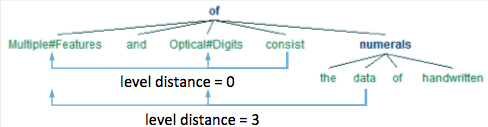
\includegraphics[width=1.05\linewidth]{figures/level-distance.png}
\caption{Dependency Tree Example}
\vspace{-0.3cm}
\label{fig:view}
\end{figure}

\subsection{CRF Feature Space}
Conditional Random Fields supports the use of many rich and overlapping local and layout features. In some degree, conditional random fields reduces a complex structural prediction problem to finding a good set of features to capture the intrinsic patterns of specified problem. Thus, feature selection is vital to the performance of a conditional random field model. In this section, we explore some efficient design of the feature space for the problem of dataset extraction.
\begin{enumerate}
\item \textbf{Local Features.} For each token to be predicted, we construct a neighboring window with size of 1. All neighboring tokens located in the window [-1, 1] are considered as a feature. Also the combination of the previous token and following token constitute another feature. For example, the window of token 'DBLP' is the sequence 'the DBLP dataset', then we would have 3 unigram features for each token and a bigram features for the combination of token 'the' and 'dataset'.  
\item \textbf{Part-of-Speech Tagging Features.} Each token is matched to a POS tagging, e.g, NN, VB. Similar like local features, a neighboring window with size of 2 is constructed. Five unigram features for each tag located in the neighboring window, and 4 bigram features for any two consecutive tags are constructed.  
\item \textbf{Heuristic Features.} We use a subset of features from the heuristic features in Sec. 3.2.1, including \textit{Capitol, Has-Dash, Mixed-Case, In-Figure, Position. } 
\end{enumerate}

\section{Semi-Supervised Learning of Conditional Random Fields}
The approaches discussed in Section 3 introduce a supervised learning process for dataset recognition problem. In a more realistic scenario, we are to start with a small set of seed items( in this case, labeled datasets and documents) and iteratively grow it by finding new contextual patterns that extracts the set of seeds from the texts. Here we show how to extend conditional random fields model to such an semi-supervised (bootstrap) learning process. 

\subsection{Seeds Selection Criteria}
For each iteration in the semi-supervised learning process, CRF labeled a new set of candidates as datasets from the testing data. There exist some false predicted datasets in the intermediate results. Thus it would be in trouble if we take all the predicted datasets as new seeds for next iteration, since the mis-labeled datasets will lead to extracting some incorrect contextual patterns in next phase. What's more, this mis-labeled error will continue to grow and finally result in a totally low performance prediction model as the iteration repeats. On the other hand, at the beginning of start point, we are only given a small set of seeds, which further means the contextual patterns found by these seeds are limited. Thus datasets appeared in previous unseen patterns will be false predicted. Therefore, at the end of each iteration, an empirical question is how to choose the subset of new seeds which would not introduce many mis-labeled errors and also make it more probable to find new contextual patterns in next iterations. 

Two evaluation metrics are purposed to balance the choice of reducing the mis-labeled error and finding more contextual patterns. First, conditional random model will generate a probability score for each predicted word. This probability score represent the confidence of the prediction result, thus could be measured as the probability of mis-labeled error. One straightforward strategy for seeds selection is to pick some predefined percentage of labeled datasets with highest confidence score. 

Second, we purposed a novel evaluation metric, called \emph{Pattern Contribution Score}, to measure the contribution of certain predicted datasets to finding new contextual patterns. Remember in Sec 2.2, for each feature function $f_k$, we use $F_k(s, o) = \sum_{i}^n f_{k}(s_{i-1}, s_{i}, o, i)$ to denote the sum of the feature counts over input sequence and state sequence. Contextual patterns are implied by these feature counts, thus a feature function with higher feature counts means its corresponding pattern is more influential to help recognizing new datasets. At the end of each iteration, our work is to select the datasets contributing to the feature functions with low feature counts, thus to find some previous unseen patterns. Aiming at this objective, we define the \emph{pattern contribution score} as follows. For each predicted dataset $d_j$, we compute the increase of feature counts over all feature functions $\{ f_1, f_2, ... ,f_m\}$, thus $\Delta I_j = (\Delta F_1, \Delta F_2, ... ,\Delta F_m)$. In each iteration, we maintain a vector of feature counts over respective feature function as $F = (F_1, F_2, ..., F_m)$. The \emph{Pattern Contribution Score} \textbf{$s$} is measure the KL Divergence Score of distribution vector $F$ and $\Delta I_j$:
\[
	s_j = D_{KL}(\Delta I_j \| F) = \sum_{k=1}^m \Delta I_j^k \ln \frac{\Delta I_j^k}{F^k}
\]
The KL Divergence Score measures the differences between two probability distributions. A higher pattern contribution score means more differences between $\Delta I_j$ and $F$, thus is more probable to find new contextual patterns. The above two metrics (\textit{Confidence Score} and \textit{Pattern Contribution Score}) emphasize on either reducing the mislabeled error or finding new contextual patterns. How these two factors balance is an empirical question we explore.

\subsection{Adaptive Training}
Once we have chosen a 'best' set of seeds, the next question to resolve is how to efficiently retain the CRF model by incorporating these new instances. A naive approach to repeat the training process would waste unnecessary computation resources. As an alternative, the intermediate statistics in each iteration are stored and utilized for future training. 
\begin{comment}
For conditional random fields, we use some gradient descent based approaches (i.e, L-BFGS) to iteratively update the parameter values:
\begin{align*}
	\frac{\delta L}{\delta \lambda_k} & = \left( \sum_j^{N_i} F_k(s^j, o^j) \right) - \\
							& \left( \sum_j^{N_i} \sum_s P(s|o^j) F_k(s, o^j)\right) - \frac{\lambda_k}{\sigma^2} 
\end{align*}
\end{comment}
In each iteration $i$, we keep records of the intermediate data $\sum_j^{N_i} F_k(s^j, o^j)$ and $\sum_j^{N_i} \sum_s P(s|o^j) F_k(s, o^j)$. In the next iteration $i+1$, we could update the corresponding terms as follows:
\begin{align*} 
	\sum_{j=1}^{N_{i+1}} F_k(s^j, o^j)  = \sum_{j=1}^{N_i} F_k(s^j, o^j) + \sum_{j=N_i}^{N_{i+1}} F_k(s^j, o^j) 
\end{align*}
\begin{align*}
\sum_{j=1}^{N_{i+1}}  \sum_s P(s|o^j) F_k(s, o^j) & = \sum_{j=1}^{N_i} \sum_s P(s|o^j) F_k(s, o^j)\\
		&+ \sum_{j = N_i}^{N_{i+1}} \sum_s P(s|o^j) F_k(s, o^j)
\end{align*}
Substituting these expressions into Equation () yields an adaptive training method for conditional random fields model. Another strategy of adaptive training is to use the learned weights $\{ \lambda_k^i \}$ in iteration $i$ as the assignments for initial values of $\{ \lambda_k^{i+1}\}$ in iteration $i+1$.

\section{Results and Discussions}
\subsection{Experiment Settings}
\textbf{Dataset.} We crawled all papers published at KDD\footnote{http://www.kdd.org/conferences} conference from year 2000 to 2012 via UMD library account. This dataset consisting of approximately 2000 academic papers is partitioned into 13 chunks by year. Chunks are iterative used as testing data in the reverse chronological order, thus from 2012 to 2000. We manually labeled datasets in the KDD 2012 papers as seeds to start the semi-supervised learning process. In each iteration, we use the previously trained chunks as training data, and a new chunk as testing data. Due to the huge efforts of munually labeling datasets to calculate evaluation metrics(i.e, precision), at current stage, we only use KDD 2011 and 2012 papers as experimental datasets. The papers in source \emph{pdf} format are converted into raw texts, tokenized and preprocessed as described in Section 3.1. \\
\textbf{Implementation.} We used CRF++ (version 0.058)\footnote{http://crfpp.googlecode.com/}, a customizable implementation of CRFs for segmentation/labeling of sequential data, and set maximum iteration to 1000 in our experiments. \\
\textbf{Evalution Metric.} F1-Score is used to measure the performance of our model. 
\[
	\text{F1-Score} = \frac{2 \cdot \text{Precision} \cdot \text{Recall}}{\text{Precision} + \text{Recall}}
\]

\subsection{Approach Comparisons}
We conduct this experiment to compare the performance of our purposed approaches (classifier and CRF). We evaluated performance of different classifiers, including SVM, Naive Bayes and Decision Tree, on both heuristic features and contextual features. The results are shown in Table 1. The column header NB is abbreviation of Naive Bayes, and DT is short of C4.5 Decision Tree.

From the table, we can see the CRF model achieves an overall F1 measure of 52.8\% on the evaluation set, outperforming other classifier methods. All the classifiers on heuristic features achieve a low recall score no larger than 30\%. In the experiments, we find many candidates(true datasets) don't show the heuristic features, like in capitol form, followed by references. Thus these candidates are falsely predicted resulting in the low recall score of classifier based on heuristic features. Another interesting finding is the simple Naive Bayes model outperforms SVM and Decision Tree in terms of Precision measure. This is reasonable since most of the heuristic features are mutual independent, which matches the independence assumption of Naive Bayes model. 

For the contextual features, the classifier obtains a better recall while suffer lower accuracy. This means that the contextual structures of describing a dataset follow some implicit patterns, which could help us identify the potential datasets. On the other hand, the classifier build on contextual features increase the number of false positives(the non-dataset words are predicted as datasets). Taking heuristic features into account could improve the accuracy of recognizing a dataset. 
\begin{table}
\centering
\hspace{-1cm}
\scriptsize
\vspace{0pt}
\begin{tabular}{|c @{\hskip 0.02in}| c c c @{\hskip 0.1in}| c c c @{\hskip 0.1in}| c |} % centered columns (4 columns) 
	\hline %inserts double horizontal lines 
	 & \multicolumn{3}{c|}{Heuristic Features} & \multicolumn{3}{c|}{Contextual Features} & \multicolumn{1}{c|}{CRF} \\
	\hline
	 Metric & NB & SVM & DT & NB & SVM & DT & CRF  \\ [0.2ex] % inserts table 
	%heading 
	\hline \hline
	Accuracy & 79\% & 58.2\% & 52.7\% & 37\% & 53\% & 44\% & \textbf{63.4\%} \\
	\hline
	 Recall & 20.1\% & 27.1\% & 13.3\% & 35\% & 38\% & 32\% & \textbf{45.1\%} \\
	\hline
	F1-Score & 31.9\% & 36.8\% & 20.8\% & 36\% & 44\% & 37\% & \textbf{52.8\%} \\
	\hline %inserts single line 
	\end{tabular} 
	\caption{Performance Comparisons}
	\label{table:comparison} % is used to refer this table in the text 
\end{table} 

\begin{table}
\centering
\hspace{-1cm}
\scriptsize
\vspace{0pt}
\begin{tabular}{|c @{\hskip 0.02in}| c | c | c |} % centered columns (4 columns) 
	\hline %inserts double horizontal lines 
	  & \multicolumn{3}{c|}{Confidence Score Metric} \\
	\hline %inserts double horizontal lines 
	 Iteration & Precision & Recall & F1-Score  \\ [0.2ex] % inserts table 
	%heading 
	\hline \hline
	Iteration 1 & 63.4\% & 45.1\%  & 52.8\%  \\
	\hline
	 Iteration 2 & 87.9\% & 63.6\% & 73.8\%  \\
	\hline
	Iteration 3 & 87.6\% &  52.8\% & 65.9\%  \\
	\hline
	Iteration 4 & 89.2\% & 54.7\% & 67.8\%  \\
	\hline
	Iteration 5 & 91.0\% & 55.0\% & 68.6\%  \\
	\hline
	\end{tabular} 
	\caption{CRF Bootstrap Learning Results}
	\label{table:bootstrap} % is used to refer this table in the text 
\end{table} 

\subsection{CRF Bootstrap Learning Results}
In this experiment, we measure the performance of our bootstrapping method and its evolution in each iterations. We used the KDD paper dataset varying from year 2008 to 2012. The papers published in year 2012 are manually labeled and used as seeds to start the bootstrapping process, other papers grouped by a year correspond to the dataset used in one iteration. In the end of each iteration, we selected the predicted datasets with top-50 probability score(\emph{confidence metric}) as new seeds adding into previous seeds. We calculated the precision and recall of the inferred bootstrapping CRF model for each iteration over a random sample of 50 papers for each year and mutually annotated datasets in these papers. The bootstrapping learning results are shown in Table 2. 

As we can see, the initial iteration obtains a F-score to 52.8\% with precision of 63.4\% and recall of 45.1\%. The bootstrapping learning system consistently increase the F1-score measure of the DNR(Dataset Name Recognition) system along the iterations and finally maintain in a relatively stable level (65\%). Another interesting observation is that as the number of iteration grows, precision increases in a relatively fast speed while recall don't improve much. On the one hand, this trend claims that the DNR system is prone to mislabel a word as a dataset (false positive) at the beginning, while the number of false positives decrease as the iteration grows. This matches the mechanism behind CRF that with more features and patterns available, the inferred CRF model is less likely to falsely predict words as datasets. On the other hands, the relatively low recall score comes from many datasets appear with irregular patterns, e.g, not in capitalize form or a irregular contextual structure. Another reason for the low recall is that some datasets are described in a table structure while not appearing in the contents, of course our CRF model aiming at analyzing the raw contents will miss such datasets.

Currently, we have only implemented the bootstrapping CRF model based on the confidence score in new seed selection phase. In next step, we plan to use \emph{Pattern Contribution Score} as new seed selection criteria or trying to find a hybrid way integrating these two metrics.

\section{Conclusion}
In this paper, we leverage linguistic tools to solve the problem of dataset extraction from scientific literatures. We attempted three different approaches for extracting dataset from texts: classifier, dependency tree and conditional random fields(CRF). We evaluated these three approaches on the KDD dataset, and got F1-Measure score higher as 70\%. Based on these work, we purposed a novel algorithm to guide conditional random fields to learning in a bootstrapping process. The results shows the F1-score continues to increase and finally come to a convergence as the bootstrapping repeats.

\bibliographystyle{abbrv}
\bibliography{report}
\end{document}
